
% \renewcommand{\tablename}{Tabla}
% \renewcommand{\listtablename}{Índice de Tablas}
% \renewcommand{\listfigurename}{Índice de Figuras}
% \begin{titlepage}
% \begin{center}
% 
\includegraphics[width=0.15\textwidth]{imagenes/cinvestav}~\\[1cm]
%
% \textsc{\LARGE CINVESTAV-IPN}\\[1.5cm]
%
% \textsc{\Large Proyecto Final Modelado y Simulación}\\[0.5cm]
%
% % Title
% \HRule \\[0.4cm]
% { \huge \bfseries Dinámica Agro-Socio-Ambiental en la conservación de la biodiversidad en México mediante la regulación de la calidad de la Matriz Agrícola\\[0.4cm] }
%
% \HRule \\[1.5cm]
%
% % Author and supervisor
% \noindent
% \begin{minipage}{0.4\textwidth}
% \begin{flushleft} \large
% \emph{Autores:}\\
% \begin{itemize}
% \item[$\bullet$] Alan Osorio Orduña
% \item[$\bullet$] Sergio Naude Citalán
% \end{itemize}
% \end{flushleft}
% \end{minipage}%
% \begin{minipage}{0.4\textwidth}
% \begin{flushright} \large
% \emph{Profesor:} \\
% D. en C. Juan Carlos Martínez García
% \end{flushright}
% \end{minipage}
% \vfill
% % Bottom of the page
% %{\large \today}
% \end{center}
% \end{titlepage}
% %\newcommand{\HRule}{\rule{\linewidth}{0.15cm}}

%\pagenumbering{Roman} % para comenzar la numeración de paginas en números romanos
\section*{Resumen}
Hoy en día las reservas naturales están siendo afectadas por la actividad humana. La producción agrícola no planificada adecuadamente, genera destrucción del hábitat alterando los ecosistemas, de tal forma que en ocasiones resulta en un daño irreversible.    \\

Disminuir el impacto ambiental provocado por las zonas de cultivo cercanas a reservas naturales sin interrumpir la producción agrícola, es una de las prioridades en diferentes partes del mundo.\\

En base a estudios que sean realizados en los últimos años se piensa que la matriz agrícola es de vital importancia. Es útil ver de manera gráfica y numérica los efectos que el hombre causa en la naturaleza. Razón por la cual se recopilo información de diferentes fuentes, todas relacionadas con el cultivo de café en Chiapas. Los datos recopilados fueron almacenados en una base de datos, para después ser utilizados para el modelo matemático realizado con cadenas markovianas. A partir de los resultados obtenidos en el modelo se describe la proyección a futuro de la calidad de la matriz. Los parámetros considerados para determinar la calidad de la matriz fueron de distintos ámbitos, desde flora y fauna del lugar, hasta métodos de cultivo y compuestos de plaguicidas y fertilizantes. \\

Con este proyecto se pretende configurar los parámetros necesarios para cambiar el estado de la calidad de  una matriz a otro, o por el contrario mantenerlo en un tiempo determinado.\\

Se realizaron programas de software para visualizar y conocer el la calidad de la matriz agrícola de las zonas de cultivos con respecto a las especies que habitan en los alrededores en un tiempo especificado.\\

Para la creación y depuración del programa se usó un compilador orientado a agentes, el cual permitió ver la interacción de las especies animales con el medio.
% \newpage
% \tableofcontents % indice de contenidos
% %\addcontentsline{toc}{chapter}{Indice de contenidos} % si queremos que aparezca en el índice
% %\newpage
% %\thispagestyle{empty}
% %\listoffigures % indice de figuras
% %\addcontentsline{toc}{chapter}{Índice de Figuras} % para que aparezca en el indice de contenidos
% \newpage
% \thispagestyle{empty}
% %\listoftables % indice de tablas
% %\addcontentsline{toc}{chapter}{Índice de Tablas} % para que aparezca en el indice de contenidos
% %\newpage
% %\thispagestyle{empty}
% %\newpage


\section{Introducción}
El crecimiento urbano propicia cambios en los espacios circundantes, tales como la pérdida de áreas agrícolas y forestales a favor de los ambientes urbanizados, y cambios en las estructuras socioeconómicas relacionadas con el manejo y propiedad de la tierra.\\

Chiapas es un estado con un fuerte crecimiento pero que aún mantiene áreas forestales, que cuentan con esquemas de protección de sus bosques.\\

El efecto del crecimiento urbano es complejo y no unidireccional, pues representa una fuerte presión para el cambio de uso del suelo, pero también ha permitido la reactivación de actividades agrícolas de bajo impacto y la revalorización de las áreas forestales.\\

Chiapas es conocido por su alta diversidad de especies de mamíferos, sin embargo, en la entidad grandes extensiones de hábitats naturales han sido modificados a zonas agrícolas, lo cual se cree que disminuye la riqueza de especies.\\

Por ello, el presente trabajo tiene como objetivo determinar la riqueza de suelo en zonas agrícolas del estado de Chiapas, particularmente en las que se cultiva café. Se recopiló información de las especies de flora y fauna de la región en bases de datos del gobierno estatal y federal, así como en colecciones de literatura científicas nacionales e internacionales.

\section{Objetivos}

\begin{itemize}
\item[$\bullet$] Descripción de la dinámica espacio-temporal de los factores agro-socio-ambientales relacionados con los sistemas agrícolas que impactan la calidad de la matriz agroecológica. Mediante el empleo de dinámicas Markovianas para la descripción de la evolución de la matriz agro-ecológica y considerando la interacción de territorios aledaños mediante dinámicas de agentes.
\item[$\bullet$] Desarrollo de un simulador computacional capaz de analizar mediante sistemas de información geográfica y bases de datos disponibles el escenario del impacto de distintos tipos de manejo agrícola en diversos contextos socio- ambientales en la dinámica espacio-temporal de la matriz.
\end{itemize}

\section{Marco Teórico}
\subsection{Cadenas de Markov}
Se conoce como cadena de Márkov a un tipo especial de proceso estocástico discreto en el que la probabilidad de que ocurra un evento depende solamente del evento inmediatamente anterior. Si se conoce la historia del sistema hasta su instante actual, su estado presente resume toda la información relevante para describir en probabilidad su estado futuro.\\

Si el estado $X_n$ y los estados previos $X_1, \dots,X_{n-1}$ son conocidos. La probabilidad del estado futuro $X_{n+1}$. No depende de los estados anteriores $X_1,\dots,X_{n-1}$. Solamente depende del estado $X_n$.\\

Es decir,

\begin{itemize}
\item[$\bullet$] Para $n = 1, 2,\dots$ y
\item[$\bullet$] Para cualquier sucesión de estados $s_1,\dots,s_{n+1}$.
\end{itemize}

\begin{multline}
    P(X_{n+1} = s_{n+1} | X_1 = s_1, X_2 = s_2,\dots, X_n = s_n ) \\ =  P(X_{n+1} = s_{n+1} | X_n = s_n)
\end{multline}

\subsection{Matriz de transición}
En matemáticas, una matriz de Markov es una matriz utilizada para describir las transiciones en una cadena de Markov. Existen varias definiciones y tipos de matriz estocástica:

\begin{itemize}
\item Una matriz estocástica derecha es una matriz cuadrada cada una de cuyas filas está formada por números reales no negativos, sumando cada fila 1.
\item Una matriz estocástica izquierda es una matriz cuadrada cada una de cuyas columnas está formada por números reales no negativos, sumando cada columna 1.
\item Una matriz doble estocástica es una matriz cuadrada donde todos los valores son no negativos y todas las filas y columnas suman 1.
\end{itemize}

Un proceso de Markov en que el sistema posee $n$ estados posibles, dados por los números $1, 2, 3,\dots., n$. Denotemos $p_{ij}$  a la probabilidad de que el sistema pase al estado $j$ después de cualquier ensayo en donde su estado era $i$ antes del ensayo. Los números $p_{ij}$  se denominan probabilidades de transición y la matriz $n\times n$  $P = (p_{ij})$ se conoce como matriz de transición del sistema.\\

La suma $1\dots p_{i1} + p_{i2} + p_{in} = 1$. Esta suma representa la probabilidad de que el sistema pase a uno de los estados $1, 2,\dots, n$ dado que empieza en el estado $i$. Ya que el sistema ha de estar en uno de estos n estados, la suma de probabilidades debe ser igual a 1. Esto significa que los elementos en cualquier renglón de la matriz de transición deben sumar $1$.  Cada elemento $p_{ij}\geq0$.\\

De la misma manera, puede definirse un vector estocástico como un vector cuyos elementos están formados por números reales no negativos que suman 1. Así, cada fila (o columna) de una matriz estocástica es un vector de probabilidad, también llamados vectores estocásticos.

\section{Simulación}
Dentro de la simulación son usados dos programas principalmente. El primero de ellos es Matlab con una interfaz gráfica, el segundo es el programa de desarrollo de ambientes Netlogo.\\

La interfaz gráfica implementada en Matlab permite ingresar los datos de la matriz de transición. Cada elemento de la matriz y el vector de condiciones iniciales son introducidos manualmente por el usuario. Después mediante un algoritmo de iteraciones entre el vector de condiciones iniciales y la propia matriz de transición, se obtiene un vector de salida. Éste último nos indica en qué tipo de clasificación se encuentra la matriz.\\

Primero se introducen las condiciones iniciales en forma de vector fila. Dichas condiciones indican la calidad de la matriz en un inicio, en escala de 0 a 1, siendo 1 excelente calidad. En base a diversas propiedades con las que cuenta la matriz es como se le asignan las componentes al vector. En el presente trabajo los factores considerados fueron:

\begin{itemize}
\item Tipo de cultivo.
\item Fertilizantes y/o plaguicidas.
\item Calidad de sombra.
\end{itemize}

La Figura \ref{fig:1} muestra la interfaz en Matlab

\begin{center}
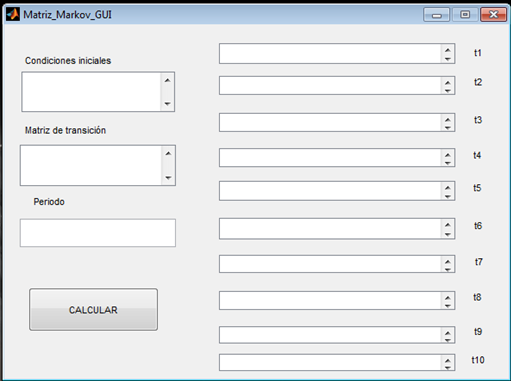
\includegraphics[scale=0.45]{imagenes/4-agricola/1.png}
\captionof{figure}{Interfaz gráfica- Matriz de Markov}
\label{fig:1}
\end{center}

La matriz de transición nos condensa las probabilidades de un estado a otro. A través de ésta matriz se puede observar el comportamiento representado por una cadena de Markov. Es decir, las propiedades de cambio entre los estados de la matriz agrícola.\\

Finalmente el periodo (en años) acota la escala de tiempo en la que se evalúa la matriz. Limitado por la información disponible, la proyección sólo se puede hacer máximo a 10 años.\\

El vector de condiciones iniciales es el siguiente:
$$\left[\begin{array}{ccc}
0{.}1&0{.}5&0{.}9
\end{array}\right]$$
La matriz de transición fijada es la siguiente:

\begin{align*}
\left[\begin{array}{ccc}
0{.}3&0{.}6&0{.}7
\end{array}\right]\\
\left[\begin{array}{ccc}
0{.}1&0{.}3&0{.}8
\end{array}\right]\\
\left[\begin{array}{ccc}
0{.}4&0{.}6&0{.}6
\end{array}\right]
\end{align*}

El programa en Netlogo muestra de manera gráfica la interacción de la matriz agrícola con especies animales. Además presenta el impacto que tienen distintos métodos de cultivo en la población de la fauna silvestre. La Figura \ref{fig:2} muestra el programa de Netlogo en ejecución.

\begin{center}
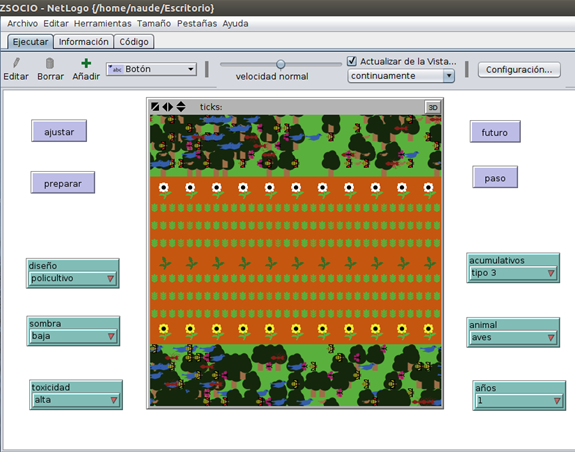
\includegraphics[scale=0.45]{imagenes/4-agricola/2.PNG}
\captionof{figure}{Interfaz en Netlogo}
\label{fig:2}
\end{center}

\section{Manual de software de simulación la calidad de la matriz agrícola de café}
\begin{enumerate}
\item Se seleccionan los parámetros de la zona agrícola.

\item Tipo de diseño, sombra, toxicidad y acumulativos.

\item Se da clic en ajustar para que muestre la zona agrícola con los parámetros deseados.

\item Se selecciona el animal con el que se pretenda visualizar como atravesara la zona agrícola con los parámetros descritos anteriormente.

\item Se presiona el botón ``preparar'' para ajustar el entorno y las variables que van estar interactuando durante el paso de la especie animal por la zona agrícola.

\item Se presiona el botón ``paso'' para que avancen cierta cantidad de espacio los animales por la zona agrícola hasta que salgan de ella.

\item Se colocan los nuevos parámetros así como la cantidad de años que a la que se quiere visualizar como se verá la matriz a tiempo futuro con los nuevos parámetros.
\end{enumerate}

\section{Conclusiones}
Se prueba la importancia de la calidad de la matriz agrícola en su entorno (en este caso es específicamente la relacionada con el cultivo de café).\\

Se visualiza de manera gráfica y numérica el impacto de la matriz con su alrededor en un tiempo finito a través de la modificación de ciertos parámetros.\\

Se encuentra la ponderación de los parámetros que puede modificar  de manera directa el hombre sobre la matriz agrícola en las zonas de cultivo de café.\\

Se logra visualizar los rangos de valores que deben tener los parámetros para reducir los daños generados por el hombre mientras realiza una actividad agrónoma,  en este caso el cultivo de café.

\bibliographystyle{ieeetr} \nocite{*}
\bibliography{bibliografias/4-agricola} %bibliografía.
